\documentclass[onecolumn, draftclsnofoot,10pt, compsoc]{IEEEtran}

\usepackage{graphicx}                                        
\usepackage{amssymb}                                         
\usepackage{amsmath}                                         
\usepackage{amsthm}                                          
\usepackage{alltt}                                           
\usepackage{float}
\usepackage{color}
\usepackage{url}
\usepackage{balance}
\usepackage[TABBOTCAP, tight]{subfigure}
\usepackage{enumitem}
\usepackage{pstricks, pst-node}
\usepackage[T1]{fontenc}
\usepackage{caption}
\usepackage{lipsum}

\usepackage{geometry}
\geometry{letterpaper, margin=0.75in}

\newcommand{\cred}[1]{{\color{red}#1}}
\newcommand{\cblue}[1]{{\color{blue}#1}}
\newcommand{\toc}{\tableofcontents}
\newlength{\drop}

\def\name{Mark Bereza}

\input{pygments.tex}

\parindent = 0.0 in
\parskip   = 0.1 in

\begin{document}

\begin{titlepage}
\begin{center}

\vspace*{50mm}

\textsc{\LARGE CS444: Operating Systems II}\\[1.5cm]

\hrule
\vspace{5mm}
{ \huge \bfseries Operating System Feature Comparison \\[0.9cm] }
\hrule 
\vspace{5mm}

\noindent
\begin{minipage}{0.4\textwidth}

\begin{flushleft} \large
\emph{Author:}\\
Mark \textsc{Bereza}
\end{flushleft}
\end{minipage}%
\begin{minipage}{0.4\textwidth}
\begin{flushright} \large
\emph{Instructor:} \\
D. Kevin \textsc{McGrath}
\end{flushright}

\end{minipage}

\vspace*{\fill}
{\large \today}\\
{\large Fall Term}

\end{center}
\end{titlepage}
  
\tableofcontents
\newpage
\renewcommand{\baselinestretch}{1.0}
\linespread{1.0}
\section{Introduction}
As the role of computers has grown from performing the same kind of calculation over and over again to a general-pupose machine that can multitask, play multimedia files, browse the web, and edit photos, the responsibilities and importance of the operating systems running on these machines has grown accordingly. These systems, often running on similar hardware and attempting to facilitate similar functionality for their end users, would often encounter similar problems and employ similar strategies to address said problems. As a result, a commmon language has arisen in the field of operating systems, making it possible to discuss or analyze different operating systems by asking questions such as "how does it avoid memory fragmentation?" or "what algorithm does it use to schedule its processes?" To aid in better understanding fundamental operating system concepts and to familiarize oneself with three of the most popular desktop operating systems in use today, this paper will ask and attempt to answer many such questions. In particular, this paper will aim to compare and contrast Linux, FreeBSD, and Windows by looking at how each implements fundamental OS functions like process scheduling, I/O, memory management, synchronization, and more.

\section{Processes, Threads, and CPU Scheduling}
Arguably the most important function of an operating system is its ability to run multiple programs simultaneously (either concurrently through the use of multiple cores or with the illusion of concurrency accomplished through a combination of time sharing and scheduling). Consequently, one of the primary responsibilities of any modern operating systems is the creation, destruction, resource management, and scheduling of multiple executing processes. While support for these basic features is ubiquitous among the three being analyzed, the actual implementation of concepts such as processes, threads, and CPU scheduling varies significantly.
\subsection{Processes and Threads}
A process, in simplest terms, is an instance of an executing program. Usually, processes have access to their own set of virtual memory independent of other processes. A thread, on the other hand, is a more granular worker employed by a process to actually perform its work. It is not uncommon for a single process to spawn and manage many threads, each sharing some common process resources to accomplish a larger common task.

In Windows, although the high-level implementation of processes and threads is fairly straight-forward, the data structures describing them and the steps needed to initialize them are extremely complex. Each process is described using an EPROCESS structure associated with at least one ETHREAD structure \cite{WindowsInternals}. Processes are created using the CreateProcess() system call, which copies some basic parameters from the calling process (affinity, I/O and page priority, security profile), but overall a new process is built from the ground up and is allocated its own address space independent of the parent process \cite{WindowsInternals}. In fact, when discussing Windows processes, using the term 'parent' to refer to the calling process is almost a misnomer since the child shares very little with the parent and by default the termination of the parent process does not impact the child. The actual creation of a process involves:
\begin{enumerate}
\item Validating parameters 
\item Opening the image file (.exe) to be executed
\item Determining the appropriate subsystem to run the image in 
\item Creating an executive process object
\item Constructing the initial thread
\item Subsystem-specific process initialization
\item Initialization of the address space
\item Scheduling/execution of the initial thread
\end{enumerate}

Below is some example code illustrating a call to CreateProcess():
\input{__createprocess.c.tex}
As you can see, despite the fact that CreateProcess() is the highest level API call for the purpose of process creation in Windows, it still allows for a multitude of input parameters. This makes sense when you consider that Windows processes, unlike those of Linux and FreeBSD, inherit very little from their parent and are mostly constructed from scratch.

The reasoning behind this lengthy and involved creation algorithm is likely a result of Windows' support for executables for various different operating systems, including MS 16-bit, DOS applications, POSIX applications, and others. Additionally, many security measures are built into this process construction procedure in order to validate debug access permissions, scheduler priority permissions, etc. This is probably a result of Windows having closed-source code and its attempt to protect the interests of developers of Windows applications. Linux and FreeBSD, on the other hand, have a far simpler process-spawning methodology using fork() because they often don't need to worry about any subsystem support and there is a lesser emphasis on restricting access to processes on the ground of proprietary information since their kernels are open-source.

The high overhead associated with spawning a new process in Windows also helps us understand the design decision to make threads the fundamental units of program execution as the overhead behind creating a new thread is far smaller.  As mentioned earlier, each Windows process is associated with at least one thread, and the threads are what actually perform the work. As a result, the Windows scheduler schedules threads, not processes. 

FreeBSD is similar to Windows in its division of responsibilities between threads and processes, though its approach to spawning new processes is more akin to Linux. A FreeBSD process keeps track of object code, global variables, kernel resources, signal state, and others. However, each process also contains references to at least one thread and, like in Windows, these are what handle execution of code. Each thread gets its own register state and stack, but beyond that threads of the same process share memory resources \cite{FreeBSD}. Threads operate either in user mode (performing work for a user application) or in kernel mode (during a system call, for example). In fact, modern FreeBSD versions map user mode threads to kernel threads in a 1:1 ratio to minimize the overhead associated with user threads frequently needing to enter the kernel. This wasn't always the case, however. Version 5 of FreeBSD and older utilized an N:M threading model; mapping potentially thousands of user threads to a far smaller pool of kernel threads \cite{FreeBSD}. The architects of this older design initially choose this approach because they envisioned the operating system frequently running server applications with thousands of users each spawning a thread that would often be idle or waiting for I/O, and thus would require far fewer kernel threads by comparison \cite{FreeBSD}. This historical insight may explain why FreeBSD, although sharing a Unix-like ancestry with Linux, differs from the latter in that it has actual support for multi-threading applications by creating a functional distinction between processes and threads. This difference is actually a good segue to discussing Linux' unique approach to processes and threads.

In Linux, although the concepts of both processes and threads still exist, there is little to no functional difference between them. In the Linux kernel, a thread is simply a process that shares memory resources with other processes. As a result, processes, not threads, are the fundamental unit of program execution and the Linux scheduler deals with processes, whether they are threads or not. To understand the reasoning behind this blatant outlier on the spectrum of process/thread implementations, two factors need to be considered: process creation overhead and historical context. 

First, let us look at process creation in Linux. Using fork() without exec() to spawn a new process allows Linux to start a new process without loading a new program, as demonstrated in the code snippet below:
\input{__fork.c.tex}

In this way, parallelization can be achieved using multiple processes with little overhead. Note that, due to fork() creating an exact copy of the parent process besides the PID, fork() can be called with no arguments, unlike the burdensome CreateProcess() in Windows. Although both Linux and FreeBSD use fork() (and its derivatives) as their primary means of process creation, in Linux both fork() and pthread\_create() simply invoke Linux's clone() system call to make a copy of the parent process. In other words, the creation of a thread and the creation of a process is virtually identical in Linux.

Additionally, processes in Linux have many of the same communication methods that are often associated with threads, such as shared memory, mutexes, semaphores, message queues, etc \cite{LinuxSlides}. Although process creation time is roughly double that of a thread, this time is still very small and the delta between the two is far smaller than on a platform like Windows \cite{LinuxSlides}. As for context switching, the overhead involved is virtually identical between threads and processes on Linux, as illustrated in the graph below:\\ \\
\begin{minipage}{\linewidth}
\begin{center}
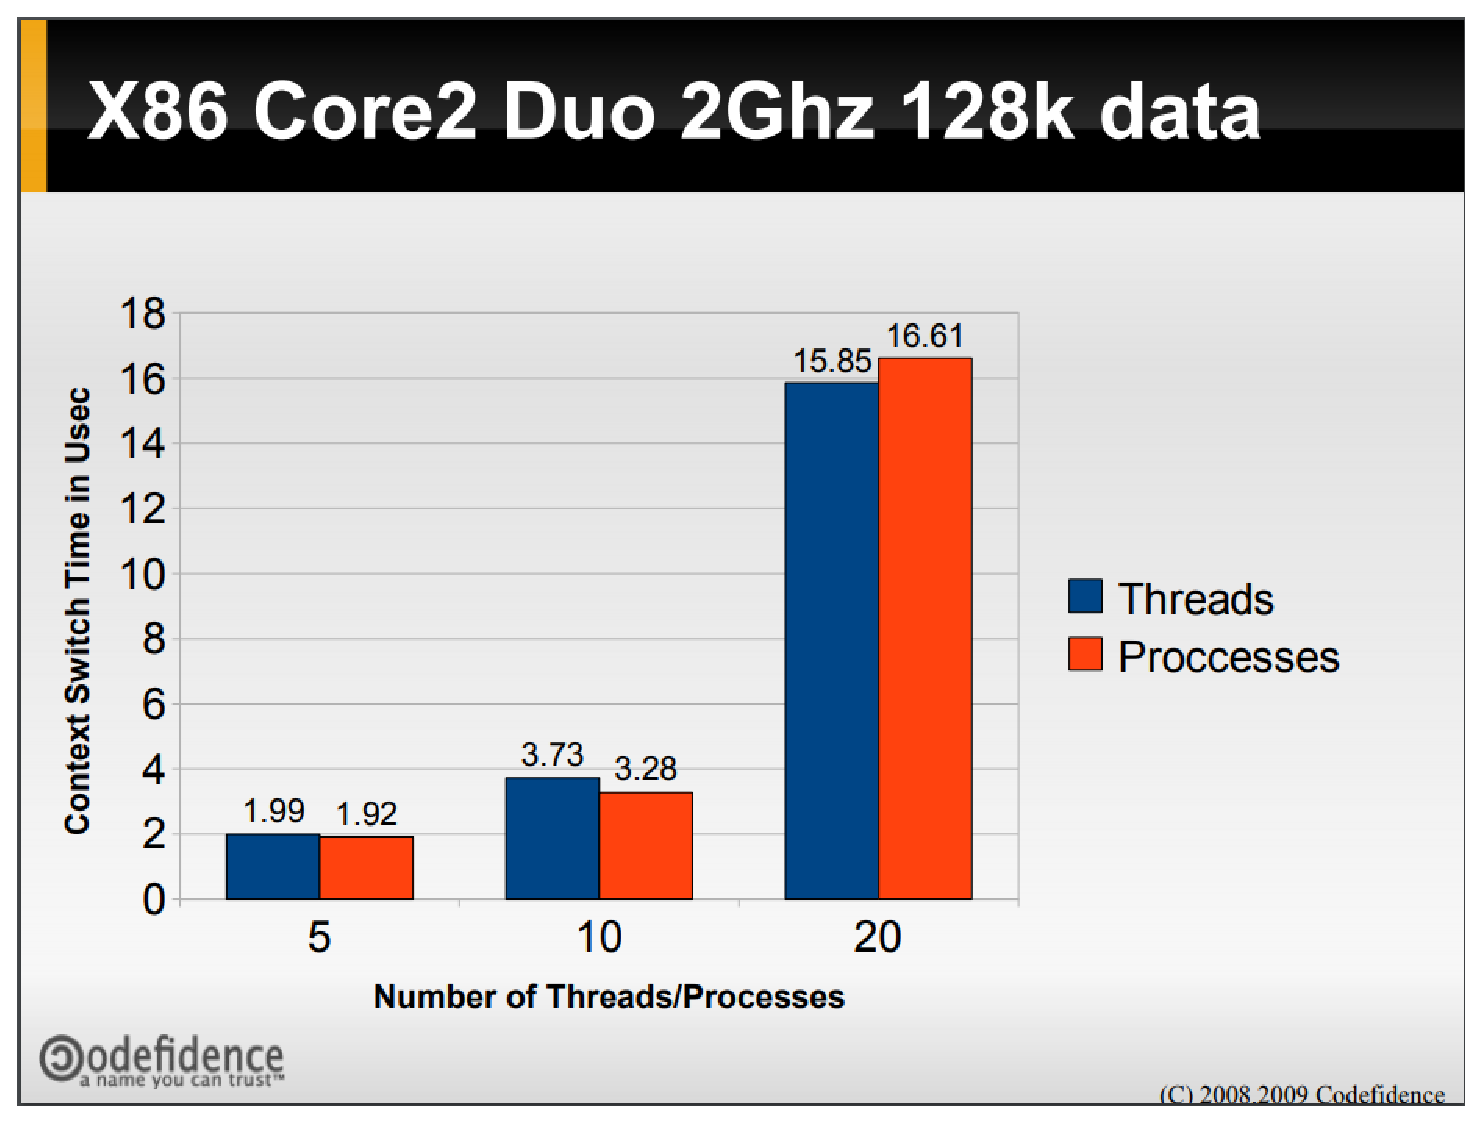
\includegraphics[width=0.6\textwidth]{context_switch_overhead.eps}
\captionof{figure}{Graph showing time it takes to context switch for both threads and processes on Linux \cite{LinuxSlides}}
\end{center}
\end{minipage}
\\ \\Thus, there is no strong case to be made from a performance perspective for why processes in Linux cannot handle the responsibilities often given to threads in other operating systems.

As for historical context, one must recall that early versions of the Linux kernel did not support multi-threading at all, treating such applications like any other normal process \cite{LinuxKernel}. Instead, the multiple lines of execution were handled and scheduled entirely in User Mode \cite{LinuxKernel}. When this old approach was deemed to be unsatisfactory as multi-threaded applications became the norm, Linux simply adapted their existing process structures to support multi-threaded applications with the use of lightweight processes.
\subsection{Scheduling}
As before, we will start with Windows. Windows utilizes a priority-driven, preemptive scheduling system \cite{WindowsInternals}. But since both FreeBSD and Linux also use schedulers that could be accurately described as being priority-driven and preemptive (in that if a higher priority thread is scheduled, the CPU context switches to it), we must dig deeper into the implementation details to uncover how these three schedulers differ. Although the functionality of the Windows scheduler, known more formally as the dispatcher, is spread throughout the kernel, it still behaves as a single entity, performing scheduling for all CPUs at all priority levels (excluding interrupts). Each thread has a priority composed of two parts: the base priority, which is a function of its process type, and the relative thread priority, which may change from thread to thread \cite{WindowsInternals}. Taken together, this priority is used to determine which threads get scheduled in what order. While a thread's base priority generally remains static, non-real-time threads can have their relative priorities changed based on a variety of system conditions. Threads of the same priority are then executed in a round-robin fashion, each running for a quanta (or time slice in POSIX terms) before giving up the CPU. 

In this sense, it is similar to FreeBSD's scheduler with a few minor caveats. Firstly, soft real-time threads are handled by a completely separate queue in FreeBSD, whereas Windows simply differentiates the soft real-time threads and normal threads via their priority level \cite{FreeBSD}. Secondly, FreeBSD additionally has a third queue specifically for idle threads, which only run on the CPU if no soft real-time or normal threads are runnable. Finally, the FreeBSD scheduler, known as the timeshare scheduler, is inherently biased in favor of interactive processes. This is because the timeshare scheduler degrades a non-real-time thread's priority whenever it consumes its time slice (or quanta) and upgrades it whenever it is idle. This means interactive processes which exhibit short bursts of computation followed by long bouts of idleness are generally given higher priority than long-running background tasks.

On the other hand, Linux's default scheduler, known as the Completely Fair Scheduler, also aims to fairly distribute CPU time, but in a different way. The CFS keeps track of a metric known as virtual runtime for each process \cite{CFS}. In essence, the less time a process has been given at the CPU, the higher its priority. This is done in order to balance CPU usage in the long term, if not the short term. Additionally, the CFS is unique among these three in its concept of sleeper fairness, or the treatment of threads that are not currently runnable as being equivalent to those on the runqueue \cite{CFS}. In this way, when said threads do finally require the CPU, the get a 'fair share', so to speak. 

Despite these slight implementation details, all three systems approach the issue of scheduling in very similar ways. All three have a soft real-time scheduling option that is treated as having inherently higher priority than default scheduling and all three utilize a "fair" scheduler for normal threads, sharing CPU time between threads of the same priority roughly equally. The key difference, then, is how much control the operating system gives the end user over the scheduling. For Windows, the answer is not very much. There is only one scheduler available that handles scheduling for every thread and it cannot be changed by the end user. Additionally, Windows even imposes restrictions on how high one can set the priority of a user-level thread, specifically requiring specific permissions to assign threads soft real-time priority. Linux, on the other hand, has a multitude of schedulers that implement different algorithms available and allows the user to assign different schedulers to specific processes. If they do not like the ones provided, they are additionally free to extend them or even create their own. Naturally, since Windows is closed-source, extensibility of existing implementations is a non-option and the wider variety of scheduler options available out of the box for Linux reflects the wider variety of environments Linux is expected to run on (all kinds of servers, mobile devices, consoles, embedded systems, etc.)
\section{I/O and Cryptography}
Another consequence of modern computers being all-purpose computation tools is that they are now riddled with various I/O devices. Thus, it is critical that any modern operating system also provides a way to interface with these devices by reading data from them and/or writing data to them. In particular, it is beneficial to create an common interface between user applications and the drivers for the I/O devices in question so that programs can access data from I/O devices without needing to know anything about how reading or writing is handled for that particular device. Additionally, many modern operating systems have begun to support cryptographic services for I/O operations to allow users to secure their data. The following section will analyze how FreeBSD and Windows implement these various services and compare them to their corresponding Linux implementations.
\subsection{I/O Abstraction}
Devices on hardware I/O buses are referenced in the Linux kernel by their I/O ports, which simply serve as numerical IDs. The Linux kernel provides auxiliary functions to simplify accessing I/O ports for reading and writing \cite{LinuxKernel}. The kernel keeps track of the mapping between specific I/O devices and I/O ports through structures called resources \cite{LinuxKernel}. These structures contain a range of I/O port addresses and are organized in a tree-like fashion to facilitate devices that are split into subsubsections. Like most things in Linux, I/O devices are represented as files (called device files) that usually live in the /dev/ directory. The advantage here is that the same system calls used to interact with regular files (\verb`read()` and \verb`write()`, for example) can also be used to access I/O devices. In order to make these generic system calls provide the specific functionality in the device, the Linux kernel employs a Virtual File System (VFS). The VFS serves as the middleman between user file operations and the device drivers; it converts system calls into the appropriate device functions \cite{LinuxKernel}.

FreeBSD, also being UNIX-based, is similar in many ways. FreeBSD also does not distinguish much between regular files and I/O device files (called special files in FreeBSD) at the user level. In fact, all I/O devices are abstracted to function as a simple stream of bytes, also known as an I/O stream. I/O streams are referenced using descriptors and these descriptors are also used to refer to everything from files, pipes, sockets, cryptographic hardware, shared memory, and more \cite{FreeBSD}. Like Linux, these special files can be accessed using the \verb`read()`/\verb`write()` system calls used to access conventional files. Unlike Linux, where the files point directly to I/O devices, all files in FreeBSD (both regular and special) point first to vnodes, which is part of FreeBSD's visualization layer. Vnodes are used to describe various file system implementations in a generic way. That being said, Linux has its own version of vnodes known as generic inodes so the differences here are minimal.

Windows, on the other hand, utilizes a service known as the I/O manager to serve as the glue between user applications, kernel services, and device drivers. This manager defines the model for I/O requests that are delivered to device drivers in a Windows system \cite{WindowsInternals2}. The specific model used by the manager is an object called an I/O request packet, or IRP, which completely describes the I/O request \cite{WindowsInternals2}. The I/O manager constructs these packets for each I/O operation and passes them to device drivers which then perform the requested I/O operations. The drivers then pass back the IRPs to the I/O manager, which will dispose of the them if it determines that the request has been completed. Moreover, the I/O manager exports common functionality to drivers, such as access to other drivers, I/O request buffers, timeouts, and filesystem data reporting to simplify driver development. This relationship between drivers and the kernel is quite different than Linux's, and is likely a result of Windows outsourcing driver development to device manufacturers using the Windows Driver Model (WDM), whereas the Linux kernel is distributed with the drivers included. This difference itself is a clear result of Windows being a closed-source microkernel, while Linux employs an open-source monolithic kernel. 

Windows threads perform their I/O operations on virtual files in a fashion very similar to how Linux and FreeBSD treat I/O devices as files. This similarity is likely a consequence of the developers of all three systems seeking to employ abstraction to simplify things for users and developers. That is, because applications either do not want to worry about or simply cannot know ahead of time the features of I/O hardware devices, a common abstract model for data reading/writing is instead provided, and that model is the file. That being said, Windows does not take the "devices are files" analogy as far as Linux does. For example, Windows does not map devices to a path in the filesystem.
\subsection{Types of I/O Devices}
Linux organizes its I/O devices intro three categories:
\begin{enumerate}
\item \textit{Block devices} are devices in which input/output operations can operate on random locations and operations are performed on integral numbers of constant-sized chunks known as blocks. Examples of I/O devices that would be categorized as block devices are RAM, hard drives, SSDs, flash memory, floppy disks, and the like. Linux performs block I/O by first passing the read/write operation to its virtual file system, which invokes the corresponding VFS function with a file descriptor and file offset. The VFS function first tries to access the data in question from the disk cache. If the disk must be accessed, the kernel determines the physical location on the device to be read/written. The kernel the uses the generic block layer to issue the necessary read/write operations to fulfill the I/O request. Since the Linux kernel operates on virtual memory, the same request may access non-adjacent chunks of physical memory and thus require multiple operations to complete. These operations are then sent to the I/O scheduler, which adds, sorts, delays, merges, and dispatches the requests based on some algorithm which aims to reduce seeking, increase throughput, prevent starvation, minimize latency, ensure fairness or some combination of these desired qualities. Finally, the requests are passed to the device drivers which actually perform the operation(s). 
\item \textit{Character devices} are devises which only allow the system to read/write sequentially. Linux in many ways treats character devices as streams of bytes. Examples include keyboards, mice, and monitors. Character I/O is often easier than block I/O because buffering strategies and disk caches are not needed.
\item \textit{Network devices}, separated from the other two categories likely because they do not map intuitively to the file abstraction, are outside the scope of this paper.
\end{enumerate}
FreeBSD, on the other hand, organizes its I/O devices into these categories:
\begin{enumerate}
\item \textit{Filesystems} read/write data to and from kernel buffers and are used to access various filesystems, as the name would imply.
\item \textit{Character devices} in FreeBSD are virtually identical to their Linux counterparts, a result of their Unix-y heritage. However, while character devices in Linux map fairly well to byte streams, character devices in FreeBSD are used to access disks and other organized data, as well. This is known as an unstructured or raw interface to a block-oriented device. I/O operations made to a disk through this interface do not go through the filesystem or the page cache. FreeBSD used to have block devices, but these were eliminated because few applications needed them and the character interface was found to improve throughput relative to the block interface. This difference from Linux is likely because Linux must support vastly more I/O devices and can run on significantly more systems and thus the flexibility provided by having interfaces for both block and character devices likely outweighs the simplicity afforded to FreeBSD by removing the former.
\item \textit{Socket devices} in FreeBSD are essentially its version of Linux's network devices and are also outside the scope of this paper.
\end{enumerate}
Windows, on the other hand, organizes its devices not based on how data is read/written, but rather based on what layer the device driver lives in:
\begin{enumerate}
\item \textit{Function devices} are the fundamental devices and each driver must implement a function driver at a minimum. It provides the operational interface for a device, including reading/writing.
\item \textit{Bus devices} represent a logical or physical bus \cite{WindowsInternals2}, such as PCMCIA, PCI, USB, etc. The bus driver will inform the Plug and Play manager of devices attached to its bus.
\item \textit{Filter devices} are essentially helper devices that augment the functionality of function and bus devices in various ways. An example of such a device would be a keylogger altering the normal behavior of keyboard operations.
\end{enumerate}
This difference in organization is likely due to Windows' microkernel approach which moves a lot of the complexity away from the core of the system and into these third-party created drivers. By creating a model that organizes different devices (and their drivers) based on where they fit in the stack, Windows can simply 'plug in' these complex drivers in their core system instead of baking in generalized functionality the way FreeBSD or Linux does.
\subsection{Cryptography}
All three of these operating systems also implement some interface for utilizing hardware-assisted cryptography, which has become more common in modern processors. This allows users to add encryption/decryption to their standard I/O operations to secure transmitted information from prying eyes. The Linux kernel has a built-in cryptography API, which provides calls for symmetric ciphers, AEAD ciphers, message digest, random number generation, and a user-space interface. A fairly basic example usage of this API can be found in \verb`/security/seclvl.c` in versions 2.6 and older of the Linux kernel:
\input{__seclvl.c.tex}
Here, a \verb`crypto_tfm` structure is used to hold an instance of a cryptographic algorithm, or transformation, and a \verb`scatterlist` structure is used to hold the block of plaintext to be transformed in a formant compatible with scatter/gather I/O. This code sets the transformation to be a \verb`sha1` encryption and then performs the following high level crypto API calls:
\begin{enumerate}
\item First, \verb`crypto_digest_init()` is called to initialize the API with the desired transformation method, in this case \verb`sha1`.
\item Then, \verb`crypto_digest_update()` takes the plaintext to be encrypted and performs the transformation on it.
\item Next, \verb`crypto_digest_final()` stores the encrypted output in the provided \verb`hash` buffer.
\item Finally, \verb`crypto_free_tfm()` deallocates the memory used to hold the transformation instance.
\end{enumerate}
As one can see, Linux uses this API to provide developers with powerful and complex encryption functionality from within the kernel using only a few lines of code.

Similarly, FreeBSD has ported the OpenBSD Cryptographic Framework (OCF), which is also an in-kernel API to cryptographic resources. This framework supports just about every common block cipher. The reason FreeBSD choose to port OpenBSD's framework instead of implementing its own like Linux is likely because FreeBSD has less support than the Linux kernel and because FreeBSD's shared heritage with OpenBSD made leveraging the existing framework a lot more attractive than writing a new one from scratch. 

Windows also has its own cryptography API, like Linux, but it is not baked into the kernel. Instead, this API instead calls upon various Cryptography Service Providers (CSPs), one of which comes included with the operating system, to allow user applications to encrypt their data \cite{WindowsCrypto}. Each CSP has its own implementation of the cryptography API layer, with some having stronger encryption algorithms than others. This difference is a result of Windows' closed-source nature, forcing it to move the cryptography layer away from the core of the system to grant users flexibility in what cryptography service they use without granting access to the system source code. Additionally, separating this complexity from the core system strengthens Windows' identity as a microkernel.

The short example program below (summarized from a longer example found on MSDN \cite{WinCryptExample}) utilizes Windows' cryptography API to encode a short message:
\input{__example.c.tex}
The flow of function calls here is fairly similar to Linux's, with \verb`CryptMsgOpenToEncode()`, \verb`CryptMsgUpdate()`, and \verb`CryptMsgGetParam()` performing functionality similar to the \verb`crypto_digest_init()`, \verb`crypto_digest_update()`, and \verb`crypto_free_tfm()` functions, respectively. The only noticable difference from the user's perspective would be the greater complexity of the Window's API, which takes more parameters, utilizes more macros, and requires manual calculation of the message size to accomplish essentially the same task. This might be due to the Linux example code leveraging the existing scatterlist structure to simplify message handling.
\section{Memory Management}
Although caching can go a long way towards reducing the number of times processes need to access memory, the fact remains that primary memory, as the name would suggest, is the memory used most by processes and the kernel itself. As a result, efficient use of primary memory, or RAM, is another fundamental responsibility for any modern operating system. The following section will analyze the different approaches to memory management taken by these three operating systems.
\subsection{Virtual Memory and Pages}
Two fundamental concepts in memory management, virtual memory and paging, are common to all three operating systems being discussed. In other words, Windows, Linux, and FreeBSD are similar in that they require that the hardware provides mapping between physical addresses and a set of virtual address that are actually used by the system. Additionally, all three operating systems are similar in the sense that the they segment the virtual address space into fixed-size blocks known as pages that map to corresponding pages in physical memory. 

Increases in the size of memory available to modern systems have pushed the addressing capacity of 32-bit systems to their limits, since such virtual address spaces can only uniquely address up to 4 GB of physical memory. For 32-bit systems, the 4 GB of virtual address space needs to be shared between the kernel and the user processes and this is where one may see the first of many differences between these three operating systems when it comes to memory management. While Linux and FreeBSD both reserve (by default) 1 GB of virtual memory to the kernel and the rest to processes, Windows splits virtual memory down the middle (by default) between the system and the user processes. This can change, however, for a process that is marked as large address aware (3 GB) or if PAE is enabled (1.5 GB) \cite{WindowsInternals2}. This difference in default behavior is likely a result of the Windows system being far less lightweight than Linux or FreeBSD and thus it would make sense for more memory to be held in reserve as a result. 

Another complication resulting from advancements in memory hardware is the size of pages themselves. While 4 KB has become the de-facto standard page size for all three operating systems, modern processors now support pages of size 2 MB and 4 MB, as well. While all three operating systems has some level of support for these non-standard page sizes (called Huge pages in Linux, Super Pages in FreeBSD, and Large Pages on Windows \cite{Hugepages}), Windows seems to be the only one of the three systems to embrace the benefits of large pages, namely the reduction in TLB overhead associated with addressing large sections of memory, by integrating their existence into standard OS memory management. Linux and FreeBSD, on the other hand, like to maintain that page size is synonymous with 4 KB. This difference is likely a result of the diverging end goals of these systems. FreeBSD is based largely on BSD, which itself is a product of academia and thus aims to be elegant and simple in design. Linux, in a similar vein, embraces singular solutions capable of addressing a wide array of use cases due to its need to run on a huge variety of hardware. Windows does not share these end goals and instead aims to simply maximize performance and usability for the most common use case in order to enhance the user experience and thus produce a better product. The added complexity needed to leverage the hardware and address all kinds of corner cases is ultimately hidden from the end users due to the closed-source nature of Windows, so this is likely not a major concern for its developers.

Another example of this difference in complexity is how each of these operating systems handle page faults, or when a process tries to access a page that has not been mapped to physical memory yet. Linux handles page faults by causing the program in question to sleep until page replacement occurs or pages are swapped out. FreeBSD simply evicts entire processes based on a Least Recently Used (LRU) page replacement algorithm. The page fault behavior for Windows, on the other hand, varies widely depending on the context of the fault. For example, if the requested page is not in memory but is on disk in the page file, the requested page is simply brought into memory. On the other hand, if the requested page is accessed from user space but is already allocated for the kernel, an access violation is raised \cite{WindowsInternals2}. 

\subsection{Page Fetching}
Two vital factors that any memory management strategy must address are when pages are fetched and when and how pages are replaced. 

When it come to page fetching, all three operating systems use some form of the demand paging strategy. Pure demand paging means that new pages are only fetched when a page fault occurs and only the requested page is fetched. The difference arises in the fact that only Linux implements a pure demand paging strategy, whereas Windows and FreeBSD implement an approximation of demand paging with some additional anticipatory paging policies \cite{Comparison1}.

Upon page fault, Windows will usually load the faulted page into memory, as would be expected from any demand paging strategy. However, Windows uses a version of demand paging known as cluster demand paging. As the name would imply, every time a faulted page would be loaded into memory, instead up to eight pages (known as a cluster) are loaded in all at once. The additional pages are often just before or after the faulted page, assuming that locality will generally mean that these pages will also be requested in the near future. Additionally, Windows implements an anticipatory fetching strategy with its logical prefetcher \cite{WindowsInternals2}. The logical prefetcher monitors the startup of the system or an application and records all page faults that occur. It then uses this information to prefetch pages it expects will be needed the next time the system or said application boots. Moreover, Windows also supports an optional feature known as SuperFetch \cite{WindowsInternals2}, a form of proactive memory management. This in particular sets it apart from both Linux and FreeBSD because this system uses historical page usage and file access information along with some heuristics to prefetch pages the system expects the user will need in an intelligent manner. The sample code provided below demonstrates how a process' memory usage may be obtained in Windows \cite{CollectMemoryInfo}.
\input{__snippet1.cpp.tex}
\par Overall, the strategy used by Windows is far more complicated than the one used by Linux, which essentially performs pure demand paging with no prefetching. This should be unsurprising since it is common for Windows, which prioritizes performance for common use cases for the average consumer over code simplicity, to use complex strategies involving data access history and multiple methods of anticipatory fetching to gain a performance edge. This is done perhaps to alleviate some of the sluggishness due to the heavy-weight nature of the OS as a whole. Linux, which could accurately be described as a kernel that is catered towards developers, seems to prioritize the simplicity of a general strategy that can handle the majority of cases adequately. This priority make sense for an open-source kernel that is maintained by a wide array of volunteer developers and Window's strategy also makes sense since its likely complicated source code is not the product they ship to customers.

FreeBSD's page fetching strategy could perhaps be described as a sort of middle ground between the Windows and Linux approaches. Although it does not utilize the complex historical usage heuristics of Windows, it does perform some level of anticipatory paging. FreeBSD, like Windows and Linux, uses the number and memory locations of page faults caused by a process over time to approximate its working set, or the subsubsection of the virtual address space that is relevant to the process at a give time period. By presuming locality of reference, the "phenomenon whereby memory references of a running program are localized within the virtual address space over short periods" \cite{FreeBSD}, the system can prefetch pages adjacent to the faulted page within the current process' working set whenever a page fault occurs. This is done to help minimize page faults and thus improve performance. Although this strategy is not much more complicated than Linux's pure demand paging, the choice to utilize some form of prefetching is likely due to FreeBSD advertising itself as being performance-conscious. While whether or not FreeBSD's claim can be substantiated is beyond the scope of this paper, it is useful to help understand its developers' decision to trade-off some simplicity in favor of better performance. The system does not take this trade-off nearly as far as Windows, and this likely because FreeBSD still ships its source code as its product, to an extent, since it is open source.

\subsection{Page Replacement}
The reason why page replacement is a very important aspect of any memory management strategy can be explained thusly:\\"Obviously, many computers do not have enough main memory to retain all pages in memory. Thus, it eventually becomes necessary to move some pages to secondary storage (back to the filesystem or to the swap space). Bringing in a page is demand driven. For paging it out, however, there is no immediate indication when a page is no longer needed by a process. The kernel must implement some strategy for deciding which pages to move out of memory so that it can replace these pages with the ones that are currently needed in memory. Ideally, the strategy will choose pages for replacement that will not be needed soon." \cite{FreeBSD}.
\par FreeBSD's implementation of page replacement is an approximation of the global least recently used algorithm, or global LRU. FreeBSD keeps track of when pages are used and uses this data to decide which page(s) should be swapped out when available memory becomes low. The global qualifier applied to this algorithm for FreeBSD simply means that any page in use by any process is a candidate for replacement. 

Similarly, Linux also implements a global LRU algorithm to determine which pages should be swapped out, but it has a caveat. Although all pages used by all processes are up for grabs, the Linux kernel separates pages into two queues: the active list and the inactive list. Pages stored in the active list are the kernel's best guess of the current working set and the inactive list contains all the other pages, which are available to be swapped.

Windows somewhat breaks away from this pattern by having implementations of both LRU and first in, first out (FIFO) algorithms \cite{WindowsInternals2}. The FIFO algorithm simply selects the page that has been in memory the longest to be swapped out. Moreover, Windows uses a combination of local and global strategies, where local simply means that the page to be swapped out is chosen only from the list of pages in use by the process that caused the page fault.

Once again, it appears that Windows is sacrificing simplicity of form for diversity of strategies that can handle different use cases efficiently. Linux and FreeBSD, which both have their roots in academia, seem to follow algorithms defined through research like LRU and demand paging more faithfully.
\subsection{Handling Memory Fragmentation}
Another issue that operating systems find themselves faced with when managing memory is how to deal with memory fragmentation, which itself comes in two flavors. External memory fragmentation occurs when unused memory exists in small chunks in between allocated memory segments. This is an issue because it makes it difficult for the operating system to efficiently provide processes with large segments of memory. Internal memory fragmentation, on the other hand, occurs due to the difference between the size of the memory provided by the system and the amount of memory actually needed by the process. With lots of requests for small amounts of memory, this can lead to most of the memory becoming unavailable despite the total amount needed by processes being relatively small.

When it comes to external memory fragmentation, all three operating systems under analysis employ a strategy known as the buddy system as a means of minimizing said fragmentation \cite{Comparison2}\cite{WindowsInternals2}. The buddy system allows an OS to provide processes with memory chunks far closer to their desired size when dealing with memory allocations smaller than a single page. It works by breaking memory into sizes of powers of two (down to some minimum granularity) and allocating the smallest amount that is at least the size requested. Every time a larger chunk of free memory is split in half to accomodate a request, the two resulting halves keep track of their corresponding "buddy". As soon as both "buddies" are freed up, they are merged back together, thus maintaining free memory in sizable continuous amounts.

In Windows, this system is not used by default when allocating memory, but is used specifically for the Low Fragmentation Heap, or LFH, one of several heap allocation strategies made available by Windows. On the other hand, both Linux and FreeBSD use the buddy system by default for allocating memory and even build slab allocators on top of the buddy system to address the other kind of memory fragmentation: internal.

In short, slabs are used both to reduce internal memory fragmentation and avoid the overhead associated with constructing objects when dealing with many objects of the exact same size. Since many kernel services deal with huge lists or trees of standardized structures, this is far from an edge case. The slab allocator preallocates a bunch of copies of a particular object continguously in memory. Whenever a process requests such an object, the allocator simply provides it with a pointer to the next available subsection and whenever a process "frees" said object, the allocator simply marks that subsection as available for later use. The primary difference between Linux and FreeBSD here is that Linux provides more options by making available for use three different slab allocators: SLOB, SLAB, and SLUB. The rationale behind the continued coexistence of these three allocators is fairly complex, but the summary is thus: SLAB was the original allocator used in the Linux kernel and is pretty close to the academic definition of slab allocation. SLUB was created as an improvement to slab; designed with modern multiprocessor systems in mind and serving as the current default. SLOB, or Simple List of Blocks, is far simpler than the other two, utilizing a simple first-fit allocation algorithm and is intended for small embedded systems \cite{SLAB}. Just from these descriptions, it is clear why Linux has this added complexity compared to FreeBSD; it is an attempt to make the kernel flexible enough to run on different types of systems, a theme that has cropped up many times now when analyzing the Linux kernel's design decisions.
\section{Interrupts and Synchronization}
As mentioned previously, the ability to properly interface with I/O devices is fundamental to any operating system. One important means of I/O communication worthy of discussion but not touched upon in the section describing I/O are interrupt signals. Since software tasks can often be completed in time spans orders of magnitude shorter than those required to complete hardware tasks, a lot of valuable processor time would be wasted if the system simply waited for a hardware task to complete before continuing. Interrupts helps to avoid this issue, otherwise known as busy waiting, by allowing the system to perform other queued-up tasks while the hardware does its job and simply context switches back to the original hardware-dependent process as soon as it receives an interrupt signal from said hardware device. In this way, interrupts (specifically the hardware kind) serve as a means of \textit{synchronization} between hardware and software.

Interrupts need not be generated by I/O devices, however. Another type of interrupt, appropriately named the \textit{software interrupt} happens at the software level. These kind of interrupts are often generated during error conditions, such as a division by zero, or during device driver service requests. Whether they are generated in hardware or in software, all interrupts break up standard process execution to perform some subroutine that handles the interrupt before returning to standard execution. 

Synchronization as a whole is important because it can ensure proper behavior when multiple processes or threads try to operate on the same write-capable resources. Mutual exclusion, the most common means of synchronizing access to shared system resources, seeks to prevent incorrect behavior resulting from race conditions by restricting access to a single thread or process during critical regions. A \textit{critical region} is any section of code that accesses shared resources in a way that cannot be executed by more than one processes concurrently.
\subsection{Interrupts}
Although both are handled by the system's trap handler, Windows make a clear distinction between exceptions, which are exceptional circumstances that occur in a deterministic manner, and interrupts, which also break up standard execution but in a non-predictable fashion. In Windows, upon receiving an interrupt signal, "the processor transfers control to a \textit{trap handler}, which is a function specific to a particular interrupt" \cite{WindowsInternals}. Before this can occur, however, the system first creates a trap frame on the kernel stack for the interrupted thread containing a portion of the thread's context, allowing the processor to switch back to it after the interrupt service routine (ISR) completes as if nothing happened. The ISRs themselves are provided by the drivers for the hardware that generated the interrupt. 

As for software interrupts, these are often generated by the kernel itself to perform asynchronous operations such as thread dispatching. Beyond the standard interrupt prioritization done by interrupt controllers, Windows "imposes its own priority scheme" on software interrupts \cite{WindowsInternals}. This scheme is known as Software Interrupt Request Levels (IRQLs) and these levels range 0 to 15 (x64) or 0 to 31 (x86), with a higher level indicating a higher interrupt priority. The highest priority software interrupt is still handled at a lower priority than any hardware interrupt, however. In the case where an IRQ comes in during the handling of another interrupt, the interrupt with the higher priority level will preempt the other. Put another way, during the handling of an interrupt with an elevated IRQL, the processor will ignore or postpone the handling of any interrupts lower than the current IRQL. Preempted interrupts are handled essentially the same way interrupted threads are; the current execution context is saved to the stack and the processor context switches back to this context after the interrupt is handled. These same IRQLs are also used to synchronize access to kernel data structures among different threads.

It is also important to note that because Windows does not allow users to control the prioritization of device IRQs and because software interrupts generated by user applications are given the lowest IRQL (passive), Windows is ultimately ill-suited for soft real-time operation despite having the process scheduling functionality for it. This is because a developer cannot make any assumptions about the worst-case delay for an interrupt request because said delays, ultimately a function of both the interrupt priority and the number of interrupts generated by higher-priority devices, are determined by the device drivers and not Windows.

Interrupts in Linux are also categorized as either software- or hardware-generated and they function in largely the same way. Following the philosophy behind its lightweight processes, the kernel control paths that Linux calls upon to service interrupts are designed to be extremely lightweight (requiring less context than standard processes) because they operate at the expense of the interrupted process in the context of scheduling \cite{LinuxKernel}. Furthermore, the Linux kernel's primary goal whenever an interrupt occurs is to return to standard execution as fast as possible in order to maintain a responsive operating system. To this end, interrupt handlers are often split into three sections: 
\begin{enumerate}
\item A critical section that must be executed immediately after the interrupt arrives and masks all other interrupts
\item A noncritical section which also executes immediately but does not mask other interrupts
\item A noncritical deferrable section whose execution may be delayed until a more convenient time.
\end{enumerate}
Just like Windows, Linux utilizes an IDT to provide mappings between interrupt vectors and their corresponding handlers. Although Linux allows for the masking and even disabling of interrupts, Linux differs significantly from Windows in that it does not assign any kind of priority to interrupts. In other words, any interrupt can preempt any other interrupt, regardless of the source. This design decision was made to both "simplify the kernel code and improve its portability" \cite{LinuxKernel}. As mentioned previously, simplicity of source code and portability across various hardware architectures are major goals the Linux kernel does not share with Windows, explaining this huge difference in implementation.

It should also be noted that the ability to move functionality into the critical section of an interrupt handler and the lack of a strict priority system make Linux far better suited to run in soft real-time operation than Windows, which is good since Linux is often used in embedded systems that benefit greatly from such functionality.

FreeBSD also handles interrupts in much the same way Linux and Windows do, with a few key differences. Firstly, unlike Windows, FreeBSD saves the entirety of the machine state to the stack before handling an exception instead of just a subset of it \cite{FreeBSD}. This is likely because the machine state maintained by FreeBSD is far smaller than the one maintained by Windows due to FreeBSD having significantly lighter and simpler processes. Additionally, unlike Linux, which uses stripped down kernel control paths to implement interrupt handlers, FreeBSD provides interrupt handlers with their own thread, stack, and context. This difference is likely a result of FreeBSD using threads as its fundamental unit of work, which are easier to construct than processes, Linux's fundamental unit of work. Moreover, unlike both Windows and Linux, which separate the scheduling of processes and interrupt handlers, FreeBSD schedules interrupts using the same system used to schedule its regular processes. FreeBSD differentiates interrupt handlers and user processes by giving software interrupts higher priority than user processes, giving hardware interrupts higher priority than software interrupts, and by allowing interrupts to preempt user processes. Overall, FreeBSD's approach to interrupts is far simpler than the approaches taken by either Windows or Linux; instead of creating a whole new system to handle interrupts, it simply leverages its existing thread structure and scheduler.  
\subsection{Synchronization}
According to \textit{Windows Internals, Sixth Edition, Part 1}, "the issue of mutual exclusion . . . is especially important for a \textit{tightly coupled, symmetric multiprocessing} (SMP) operating system such as Windows, in which the same system code runs simultaneously on more than one processor, sharing certain data structures stored in global memory." The Windows kernel accomplishes this task by providing mutual-exclusion primitives used to synchronize access to these global structures. Synchronization performed by Windows can be split into two categories: high-IRQL synchronization and low-IRQL synchronization. 

In the former, the IRQL is high enough that the synchronization must not rely any code that could result in page faults or rescheduling since the interrupts that drive these operations are not handled at this IRQL. The most difficult part of ensuring mutually exclusive access to global structures in this context is preventing interrupts interleaving their critical sections with those of the interrupted thread. On single-CPU systems, the desired mutual exclusion can be achieved by elevating the IRQL to level high enough where all interrupts that could modify the data structure in question are ignored. For multiprocessor systems, mutual exclusion is achieved using \textit{spinlocks}. Spinlocks protect shared data structures by forcing threads to wait (or "spin") until they acquire the lock for a data structure before executing any code that may modify its contents. Additionally, these spinlocks in Windows have an IRQL high enough to where the system's dispatching mechanisms are ignored, ensuring that a "spinning" thread is never preempted and thus locks are acquired and released quickly. The Windows kernel provides an interface to these spinlocks via its \verb`KeAcquireSpinLock()` and \verb`KeReleaseSpinLock()` system calls, illustrated in the code snippet below \cite{dictlib}:
\input{__spinlock.c.tex}
The snippet shows a method for allocating an entry in a shared dictionary structure. Before making any modifications to the dictionary structure, the function first attempts to acquire the dictionary's spinlock by calling \verb`KeAcquireSpinLock()` with a pointer to the desired spinlock and the current IRQL. As soon as the entry is successfully allocated, the function releases the spinlock using \verb`KeReleaseSpinLock()`, providing it the same parameters as before.

In the latter case (low-IRQL), the IRQL is low enough where page fault handling and thread rescheduling may occur. In this case, spinlocks are often too inefficient or too restrictive and a variety of other locking mechanisms are utilized instead, including kernel dispatcher mutexes and semaphores, fast and guard mutexes, pushlocks, and executive resources, whose features are outlined in Figure 2.\\ \\
\begin{minipage}{\linewidth}
\begin{center}
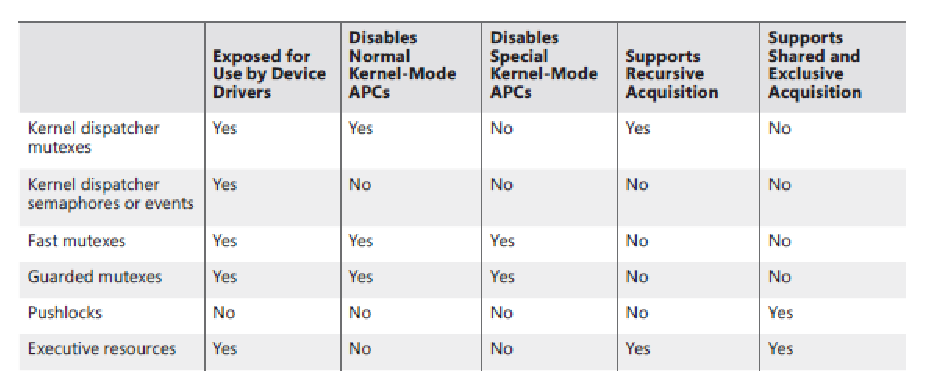
\includegraphics[width=0.8\textwidth]{table.eps}
\captionof{figure}{Table outlining the features of various Windows locking mechanisms \cite{WindowsInternals}}
\end{center}
\end{minipage}
\\ \\ Linux, lacking a priority system for interrupts, does not split its synchronization strategies along said lines and instead simply provides a series of synchronization primitives for various use cases. Here are some of the more common ones:
\begin{enumerate}
\item \textit{Per-CPU variables} simply implement a variable as an array, with one element per CPU, thus preventing race conditions when it makes sense to split a variable across each of the CPUs.
\item \textit{Atomic operations} ensure, at the assembly level, that read-modify-write operations are performed atomically, thus preventing race conditions.
\item \textit{Optimization and memory barriers} prevent the reordering of instructions before and after a synchronization primitive and also force memory operations occurring before the primitive to complete before starting operations after the primitive.
\item \textit{Spinlocks} used in the Linux kernel are essentially identical to the ones used by Windows.
\item \textit{Read-copy update (RCU)} is a lock-free synchronization method in which writers make a copy of the shared data structure, perform the writing on the copy, and update the structure's pointer to be a pointer to said copy. Because the update step occurs atomically, race conditions are avoided.
\item \textit{Semaphores} are similar to spin locks in that they force a process to block until it obtains the lock, but differ in that they force the process to sleep until the resource becomes available.
\item \textit{Local interrupt disabling} achieves synchronization on single-CPU systems by disabling interrupts during critical regions.
\end{enumerate}
While there is some overlap between the synchronization methods provided by Windows and the ones provided by Linux, the key takeaway here is that Linux provides many more options. This is likely because the priority-less, infinite interrupt nesting allowed by the Linux kernel makes having efficient synchronization methods for a wide variety of scenarios crucial to maintaining performance.

Interestingly, the term \textit{critical section} takes on a slightly different meaning in the context of FreeBSD. Instead of describing a section of code subject to race conditions, critical sections in FreeBSD are themselves synchronization constructs that prevent threads from being either migrated or preempted \cite{FreeBSD}. Although, like Linux's local interrupt disabling, they only guarantee synchronization across a single CPU, they are preferable to other locking mechanisms in that they require far less overhead. The other locking mechanisms available in FreeBSD can be found in Figure 3. 
\begin{minipage}{\linewidth}
\begin{center}
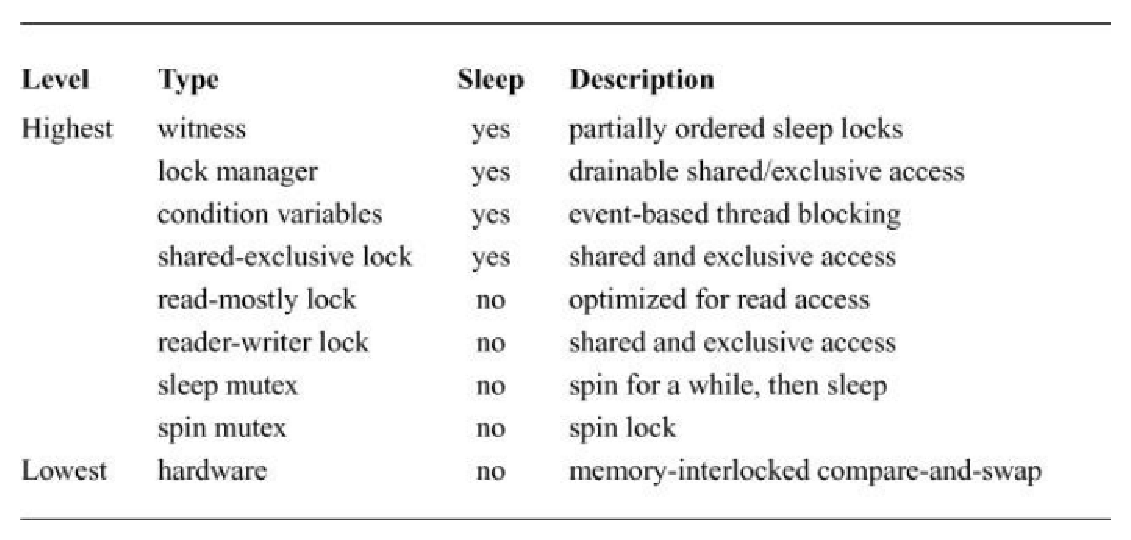
\includegraphics[width=0.8\textwidth]{table2.eps}
\captionof{figure}{Table outlining FreeBSD's locking hierarchy \cite{FreeBSD}}
\end{center}
\end{minipage}
\\ \\ The most interesting difference here is that, unlike the locking primitives of Windows and Linux, the ones provided by FreeBSD are organized into a sort of hierarchy. In fact, witness, the highest level lock, is capable of performing high-level functionality like deadlock prevention at the cost of increased overhead. The reason for this difference is largely historical; as the FreeBSD kernel codebase grew and the number of the developers increased, "the ad hoc method of maintaining the partial ordering of locks became untenable. A witness module was added to the kernel to derive and enforce the partial ordering of the locks" \cite{FreeBSD}.
\section{Conclusion}
In conclusion, although FreeBSD, Windows, and Linux all implement processes, scheduling, I/O, cryptography, memory management, and synchronization, the details of said implementations vary greatly as a result of the history of these systems, the accessibility of their source code, and the hardware platforms they aim to run on. Additionally, these differences serve to reveal the difference in the design philosophies of these systems. For example, FreeBSD, not concerned with running on the vast array of hardware Linux has to run on, was able to simplify I/O by dropping block devices altogether. Windows, seeking to prserve the integrity of its proprietary code but lacking the resources to provide drivers for every device under the sun themselves, seperates I/O drivers and crypto services from the core system and instead provides manufacturers with the interface to create their own Windows-compliant drivers. 

In other ways, these three have more in common than they do different. For example, Linux and FreeBSD's approaches to memory management are quite similar, whereas Windows implements a lot of the same concepts (LRU, demand paging, virtual memory), but in more nuanced and complex ways. As mentioned earlier, Windows prioritizes the performance of the end product over the organization or simplicity of the code base because of its closed-source nature. Thus, Windows developers are more than willing to put more burden on the code base in order to improve performance in a large variety of use cases. Linux and FreeBSD, on the other hand, utilize simple but effective algorithms that work in the general case, thus keeping their open source code base simpler. Finally, it appears that FreeBSD is willing to add some use-case specific improvements (like page prefetching) that Linux is not. This can likely be attributed to the fact that Linux aims to run on a larger range of hardware environments than FreeBSD and FreeBSD advertising itself as a performance-conscious operating system.

Overall, despite the myriad of differences in implementation details, these operating systems as a whole approach common problems like scheduling, paging, and virtual memory in very similar ways. For Linux and FreeBSD, this could reasonably be attritubed to their common Unix heritage, but this explanation ceases to function when Windows is thrown in the mix. Here, a more fitting explanation would be a sort of convergent evolution. Since these systems, being operating systems meant to run primarily on personal computers, have largely similar end goals of efficiency and performance, it makes sense that they would tend towards similar, effective strategies at the high level. 
\newpage
\bibliographystyle{IEEEtran}
\bibliography{mybib}

\end{document}
